\baselineskip=8mm
% \renewcommand{\thesubsection}{\thechapter.\arabic{subsection}}
\numberwithin{equation}{chapter}
\numberwithin{equation}{section}
\renewcommand{\thesubsection}{\arabic{subsection}.}
\renewcommand{\theequation}{\thesection.\arabic{equation}}
\renewcommand{\thesection}{}
\renewcommand{\thesubsubsection}{\thesubsection\arabic{subsubsection}.}




\section{การออกแบบส่วนเชื่อมต่อประสานกับผู้ใช้}

ในการออกแบบส่วนต่อประสานกับผู้ใช้ของแอปพลิเคชันจัดตารางเวรพยาบาลจะเน้นไปที่ความเรียบง่าย สบายตา และใช้งานได้ง่าย เพื่อให้บุคคลากรณ์ทางการแพทย์ใช้ได้ง่ายและรวดเร็ว โดยจะมีการออกแบบหน้าจอต่างๆ แบ่งตามประเภทของผู้ใช้ได้ดังนี้


\subsection{Application Admin}

\begin{figure}[h]
    \centering
    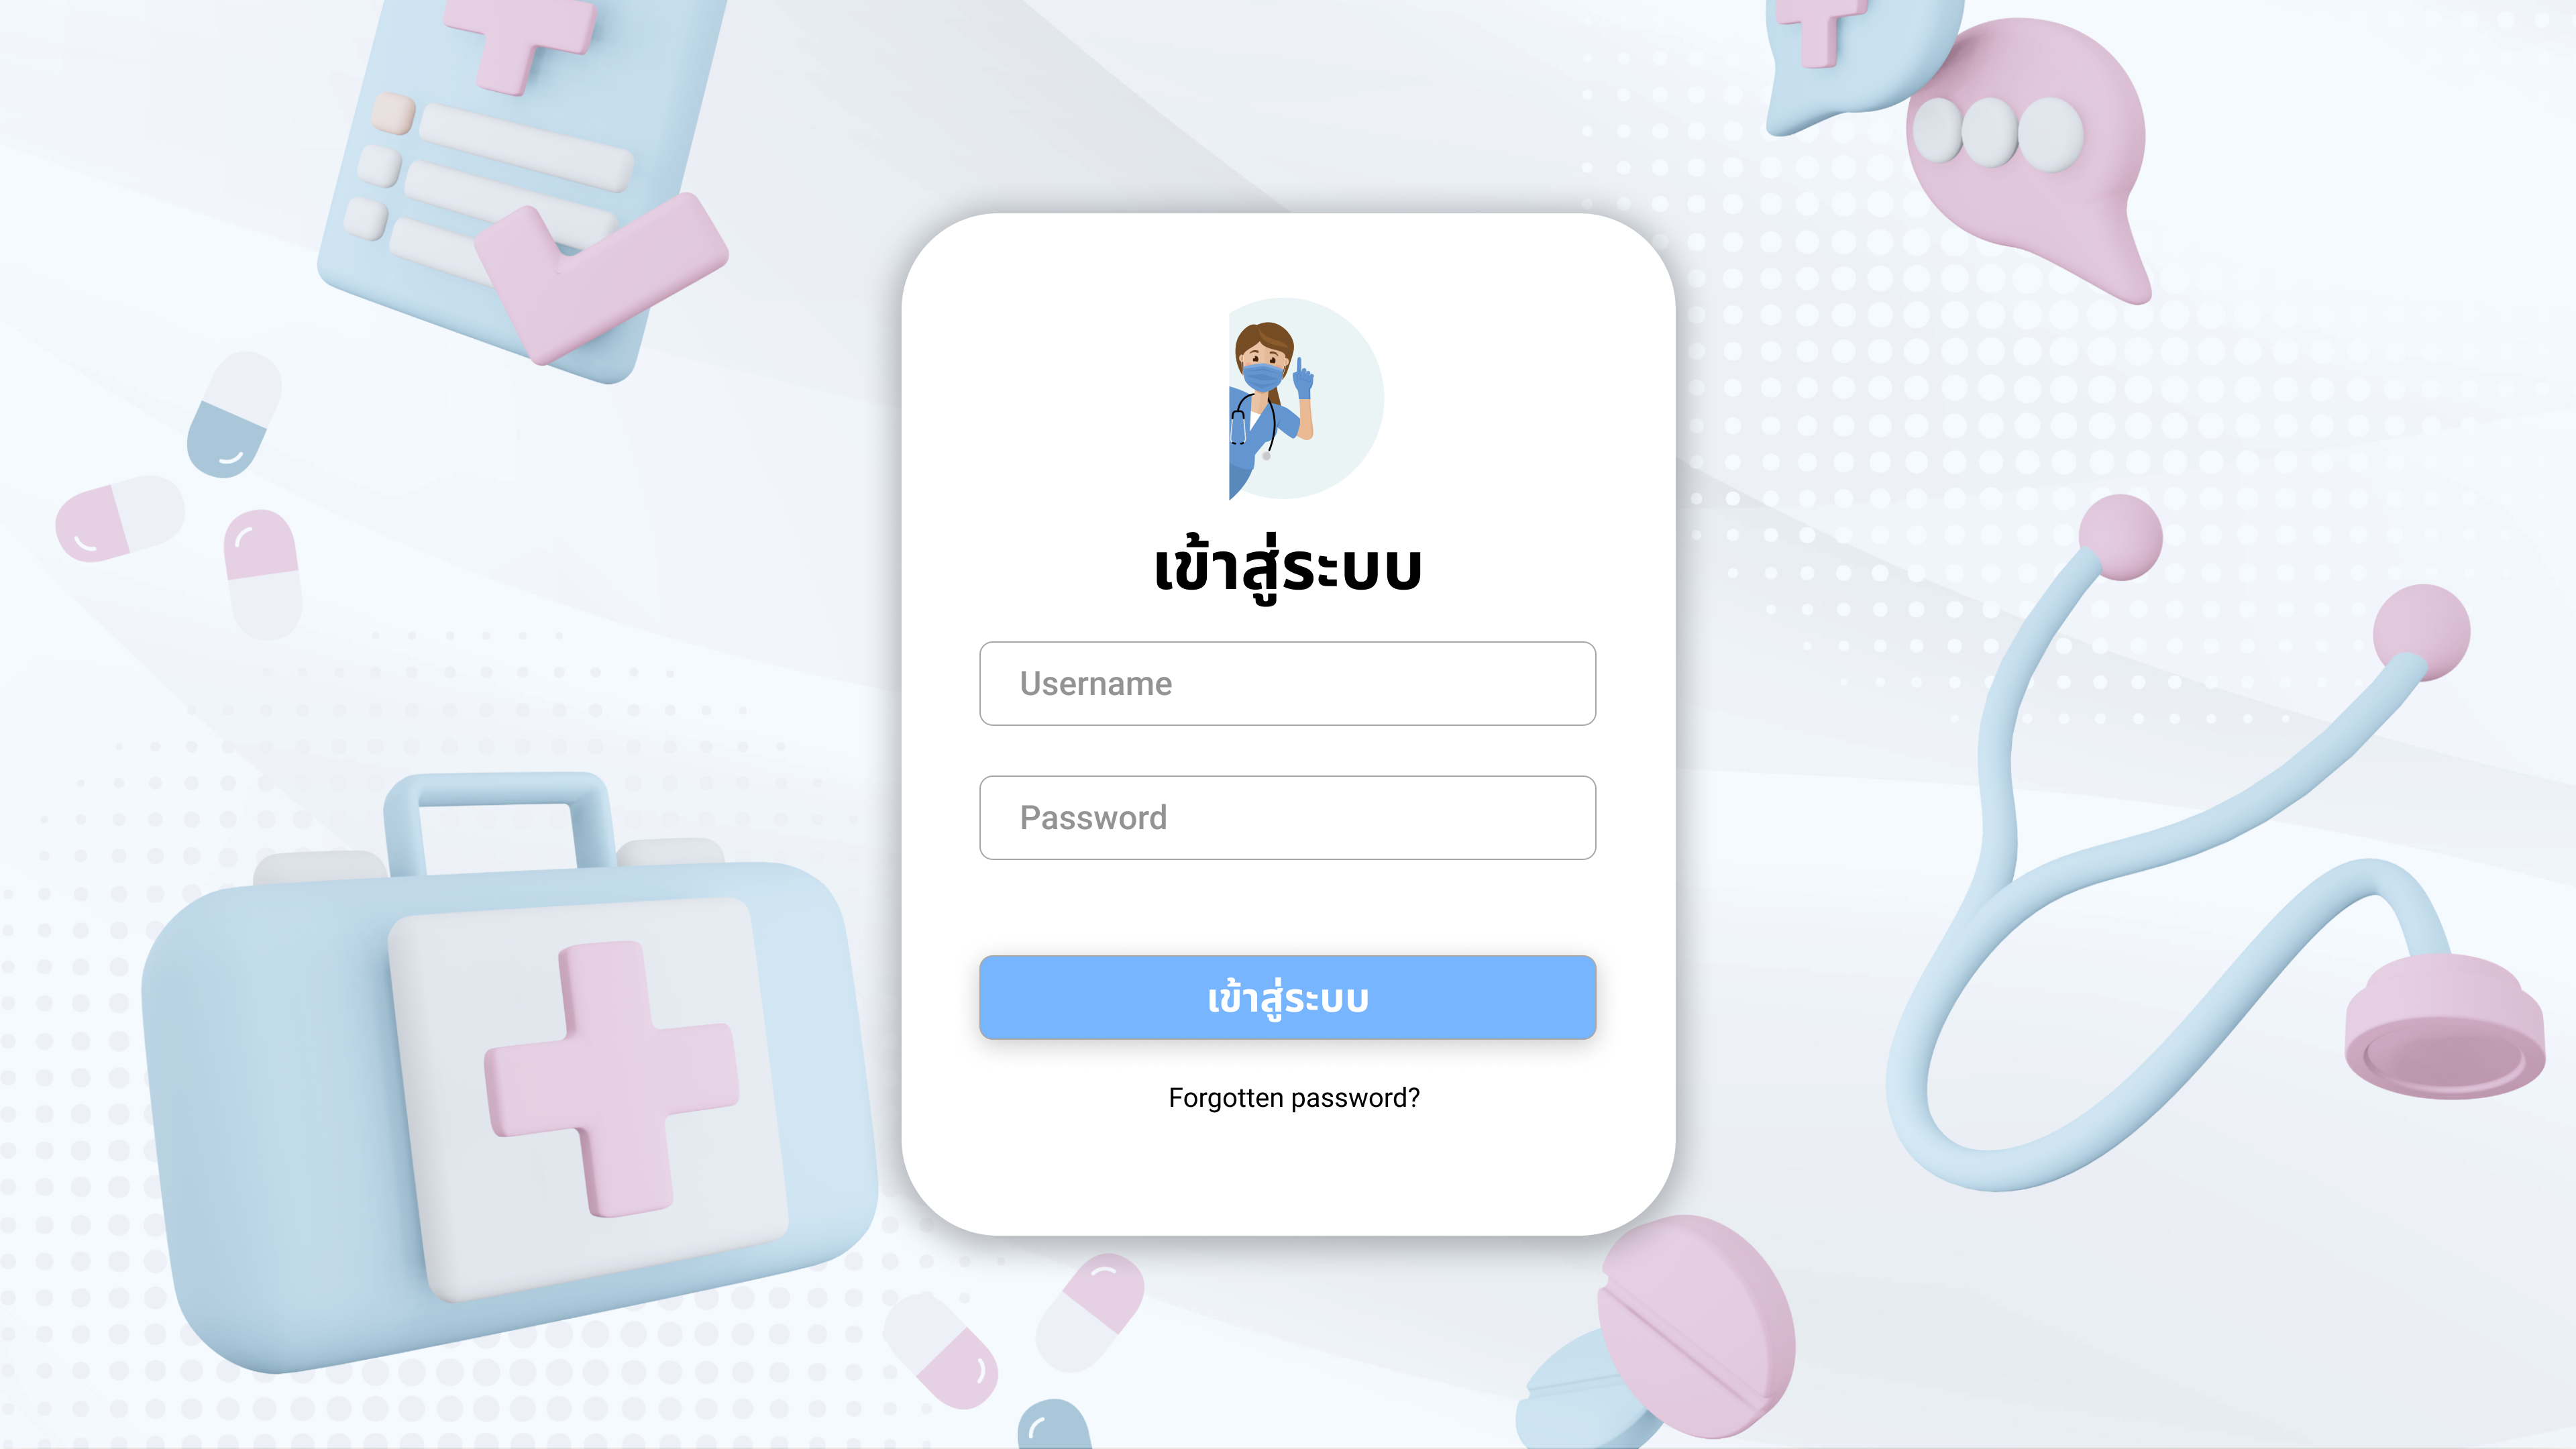
\includegraphics[width=0.6\textwidth]{Login ui.png}
    \caption{หน้าต่างการเข้าสู่ระบบของแอดมินแอปพลิเคชัน}
    \end{figure}

\subsection{Hospital Admin}

\begin{figure}[h]
    \centering
    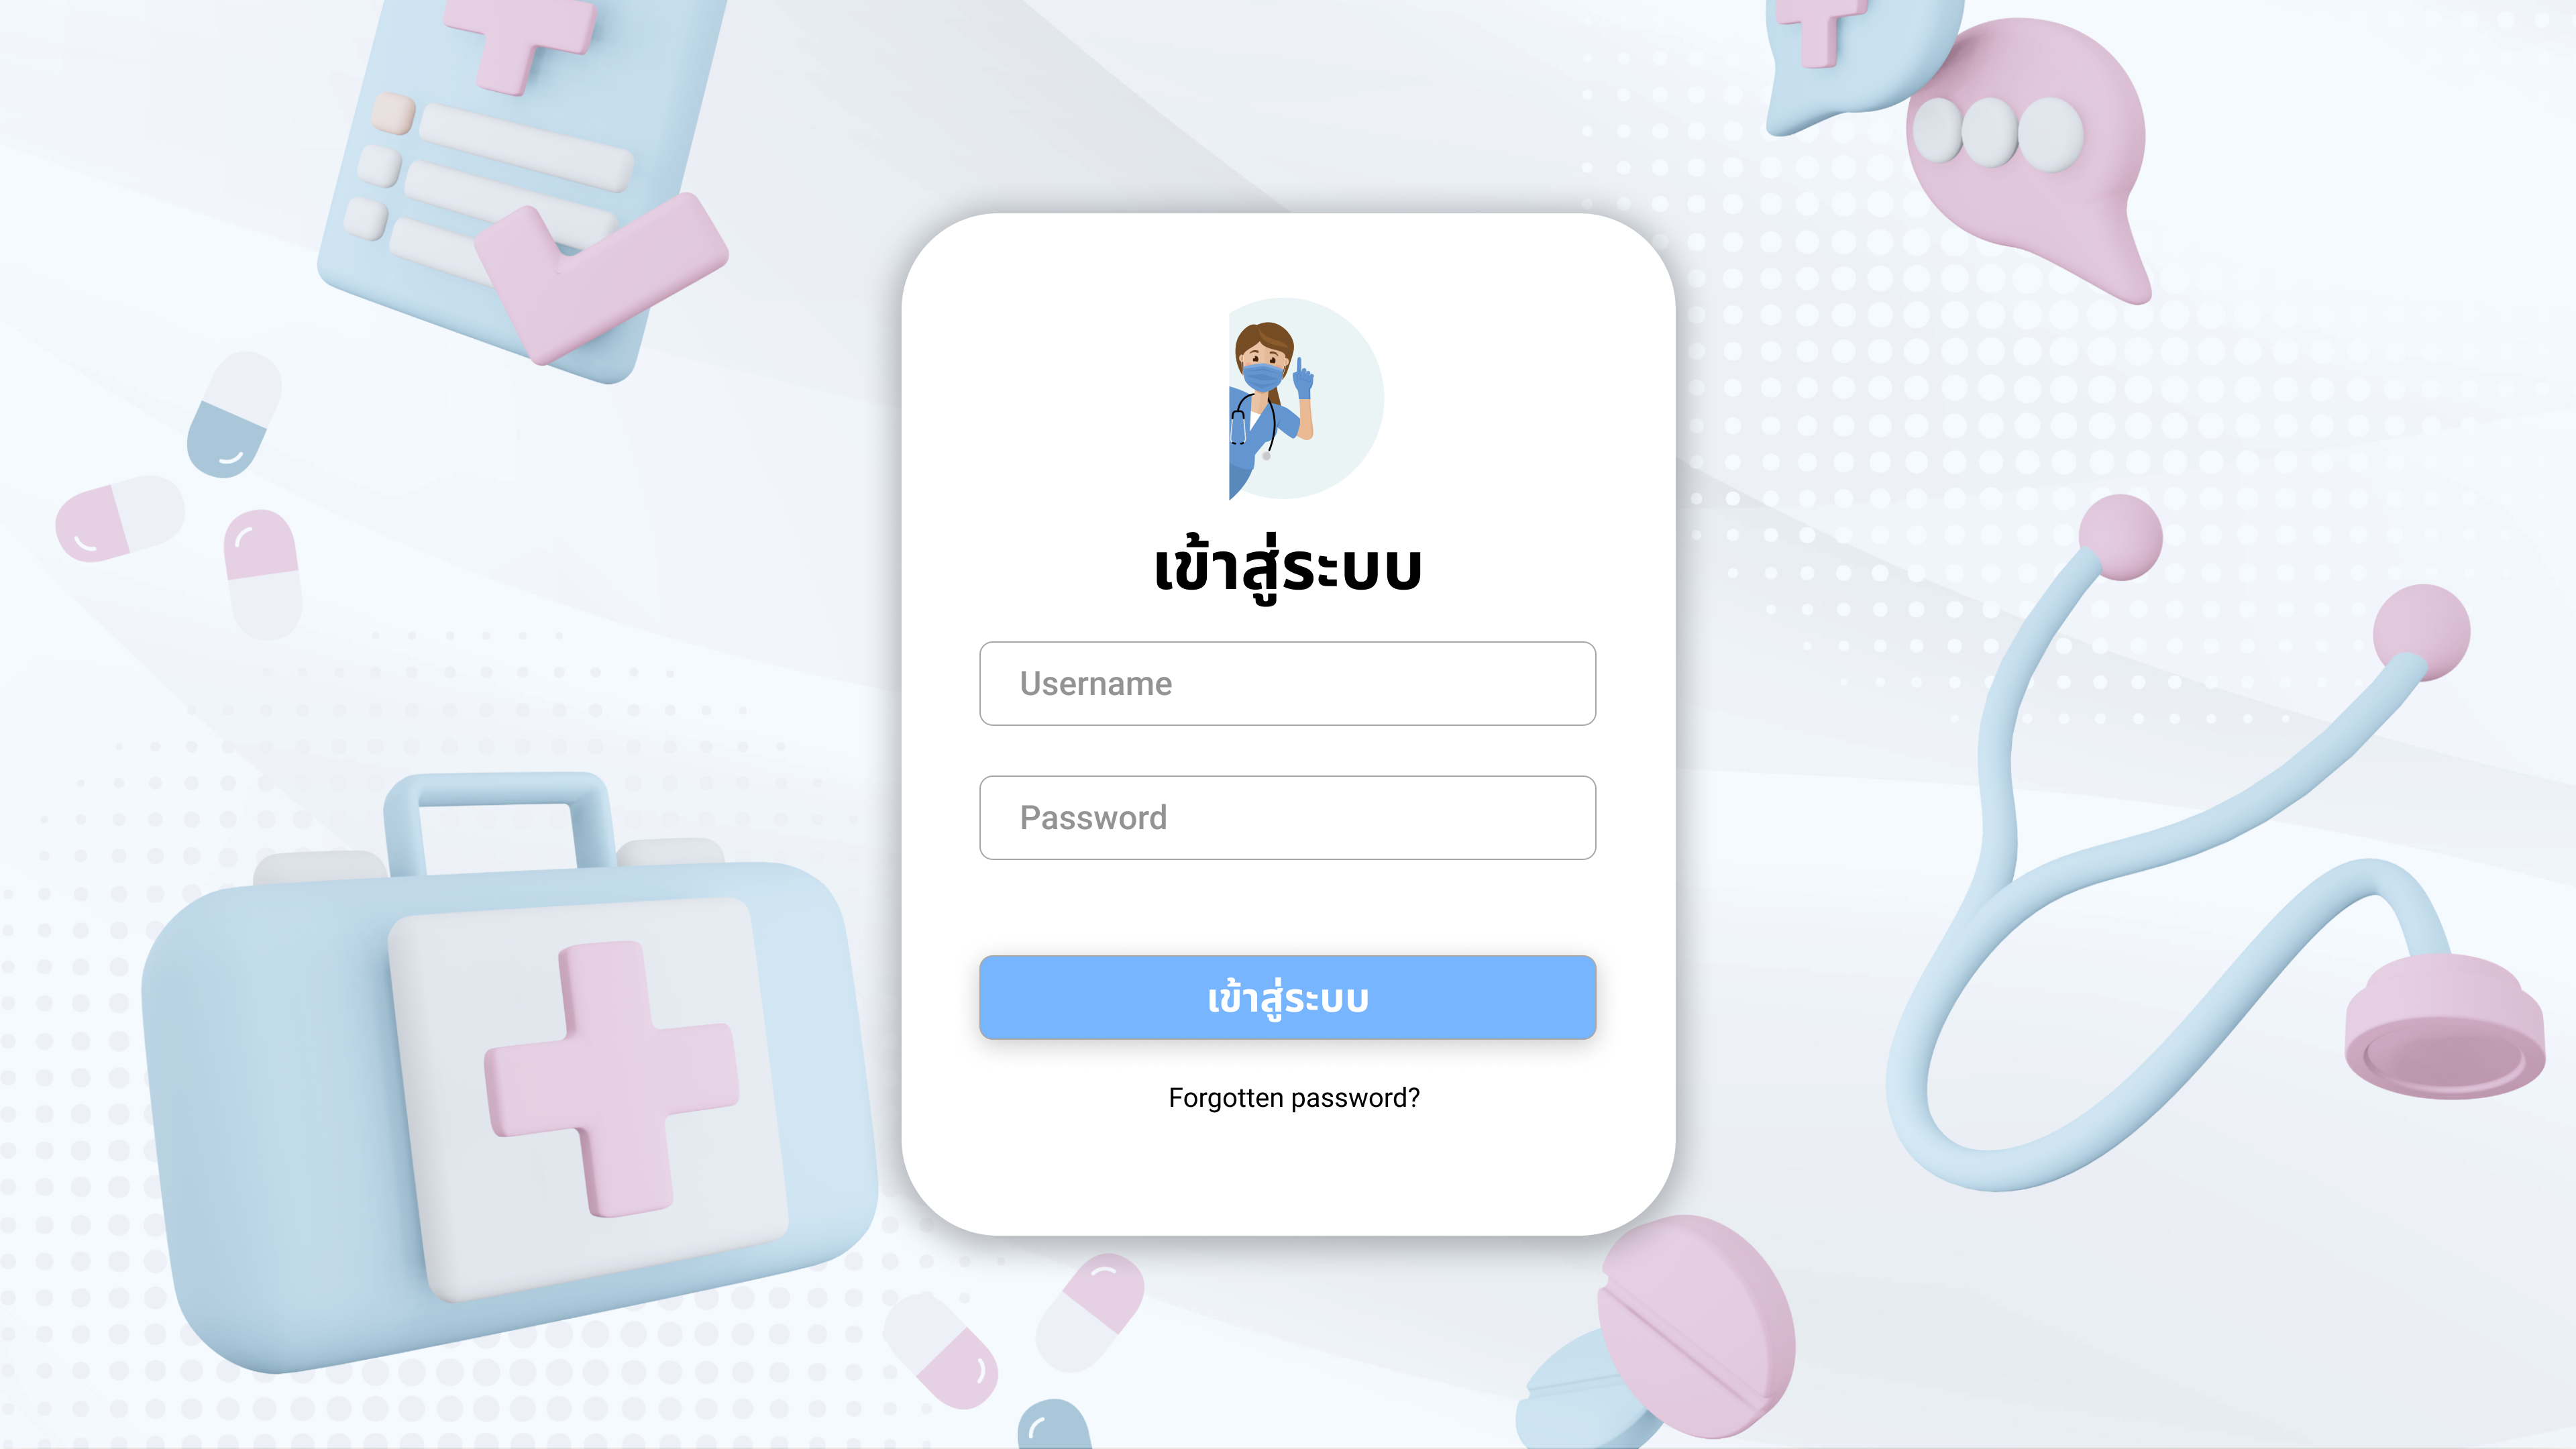
\includegraphics[width=0.6\textwidth]{Login ui.png}
    \caption{หน้าต่างการเข้าสู่ระบบของแอดมินโรงพยาบาล}
    \end{figure}

\subsection{Hospital Director}

\begin{figure}[h]
    \centering
    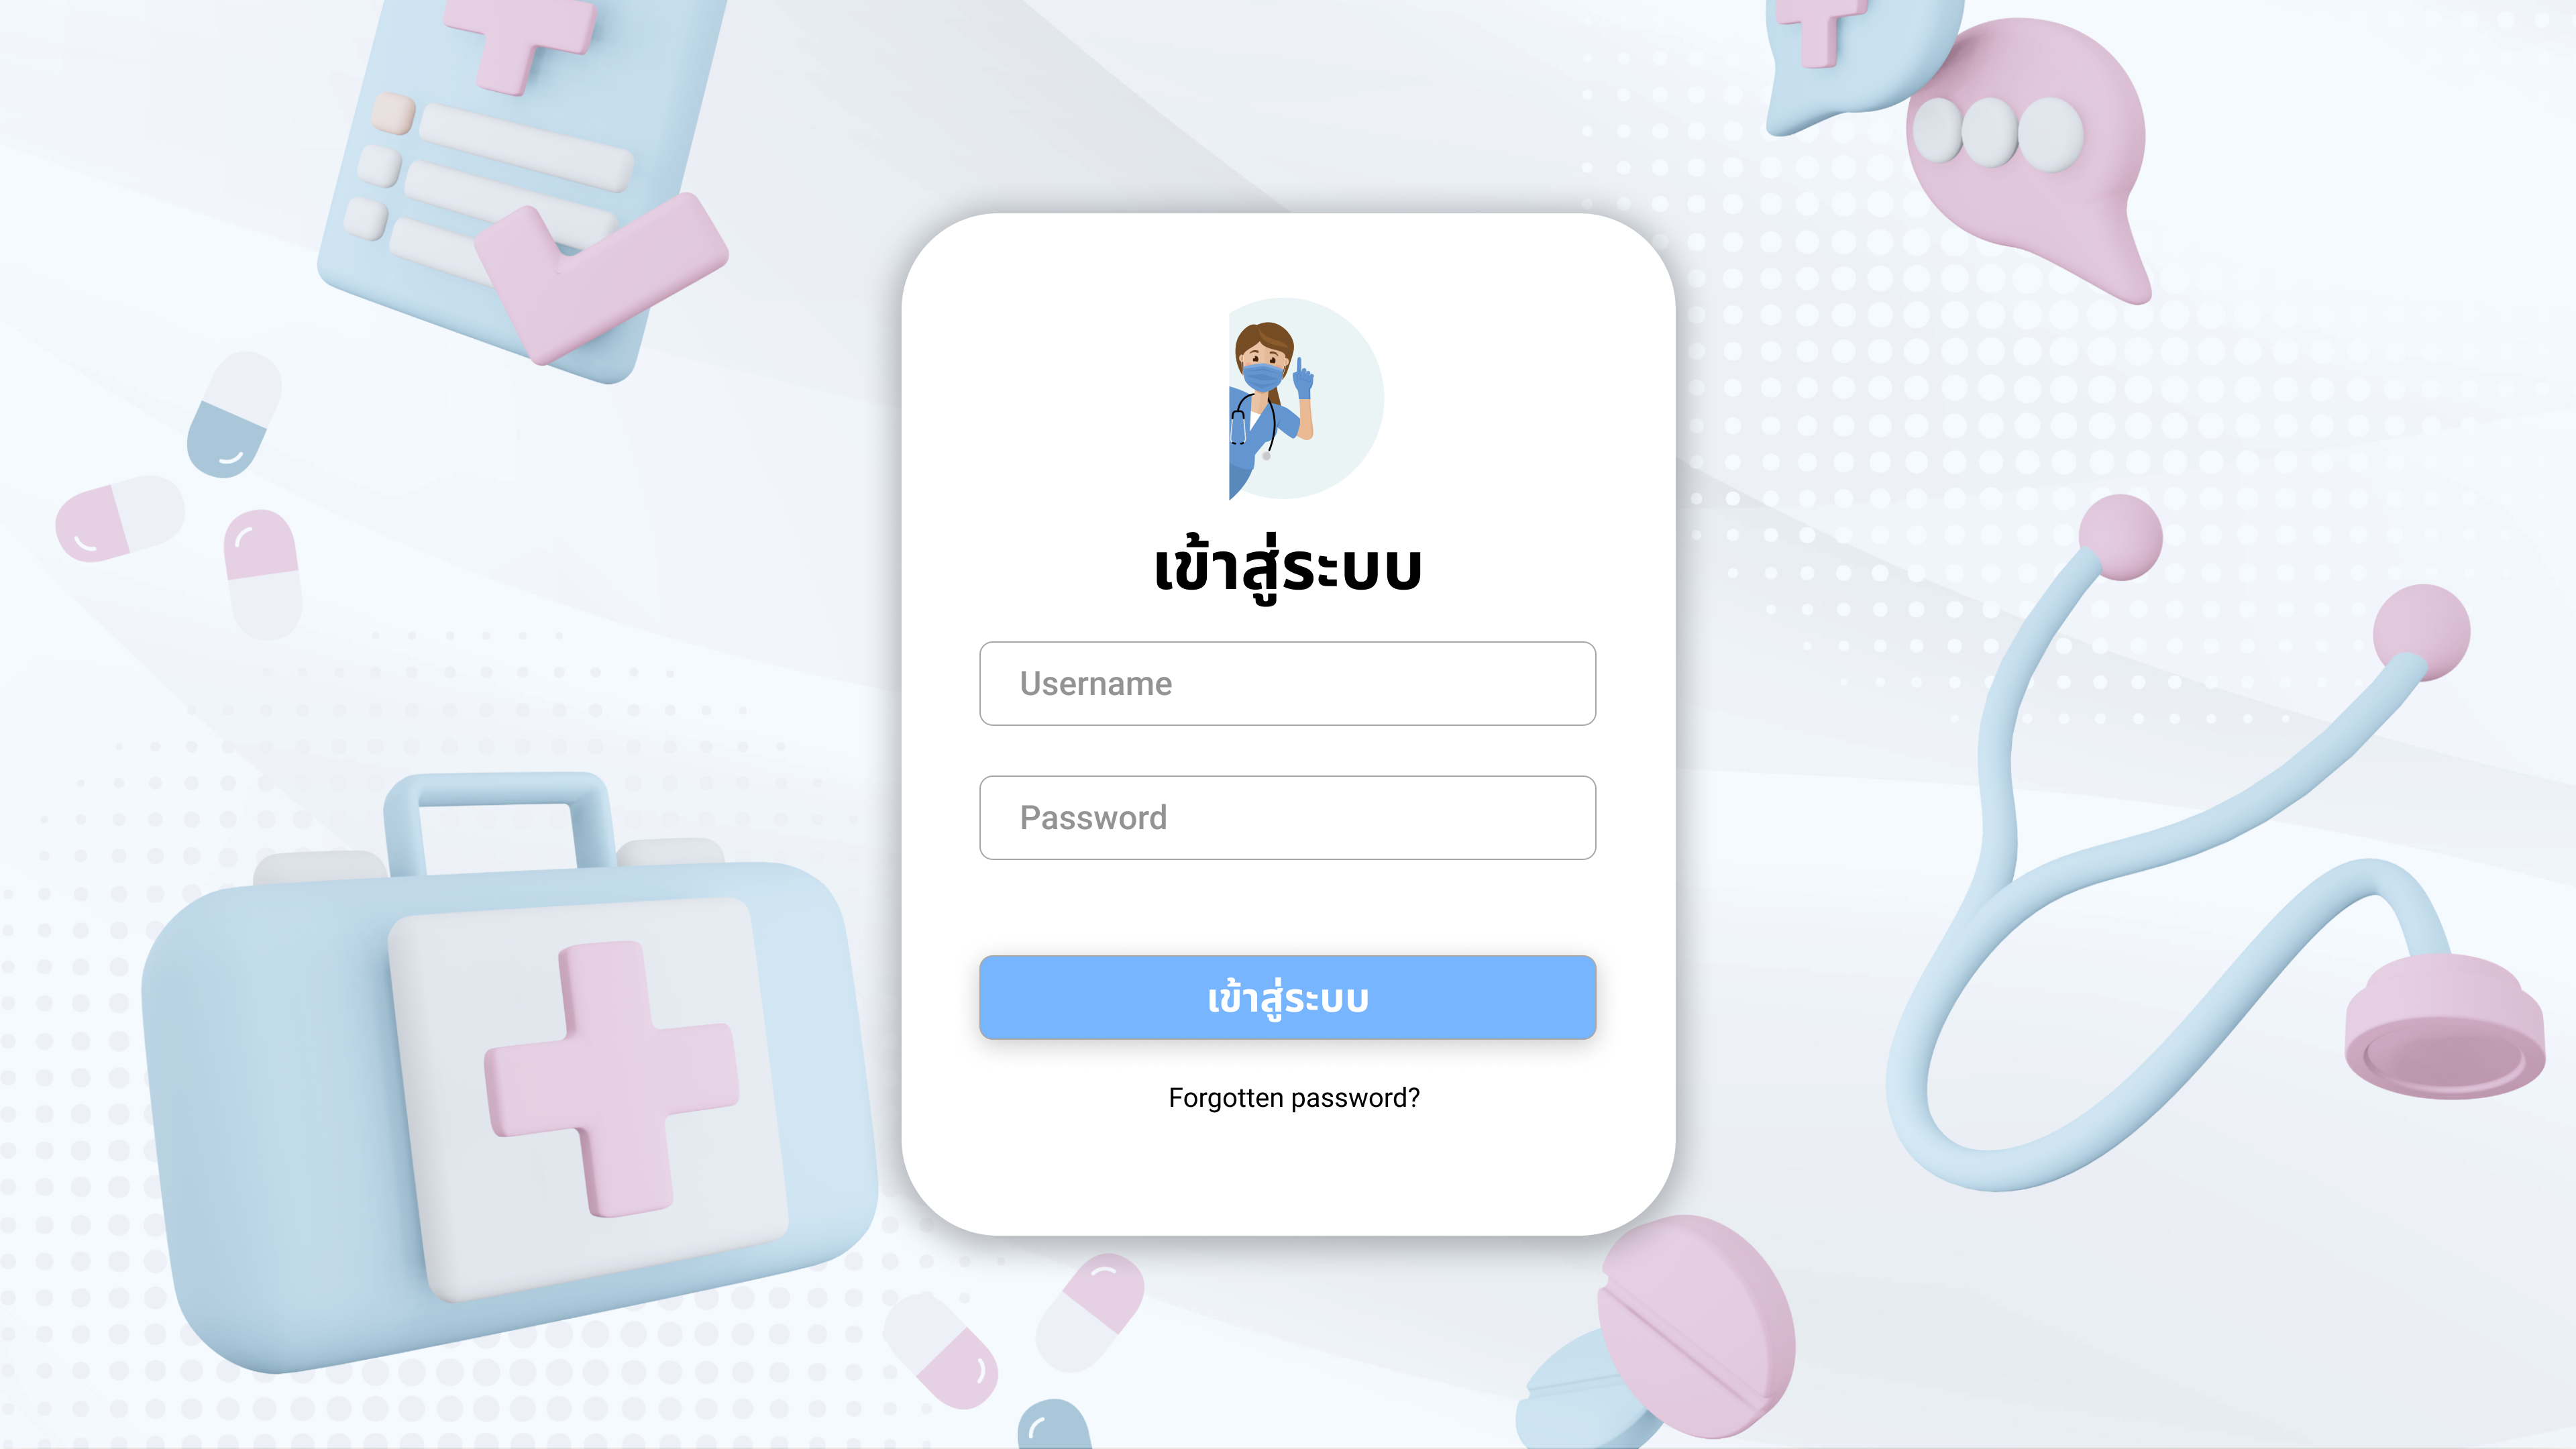
\includegraphics[width=0.6\textwidth]{Login ui.png}
    \caption{หน้าต่างการเข้าสู่ระบบของผู้อำนวยการโรงพยาบาล}
    \end{figure}

\subsection{Headnurse}

\begin{figure}[h]
    \centering
    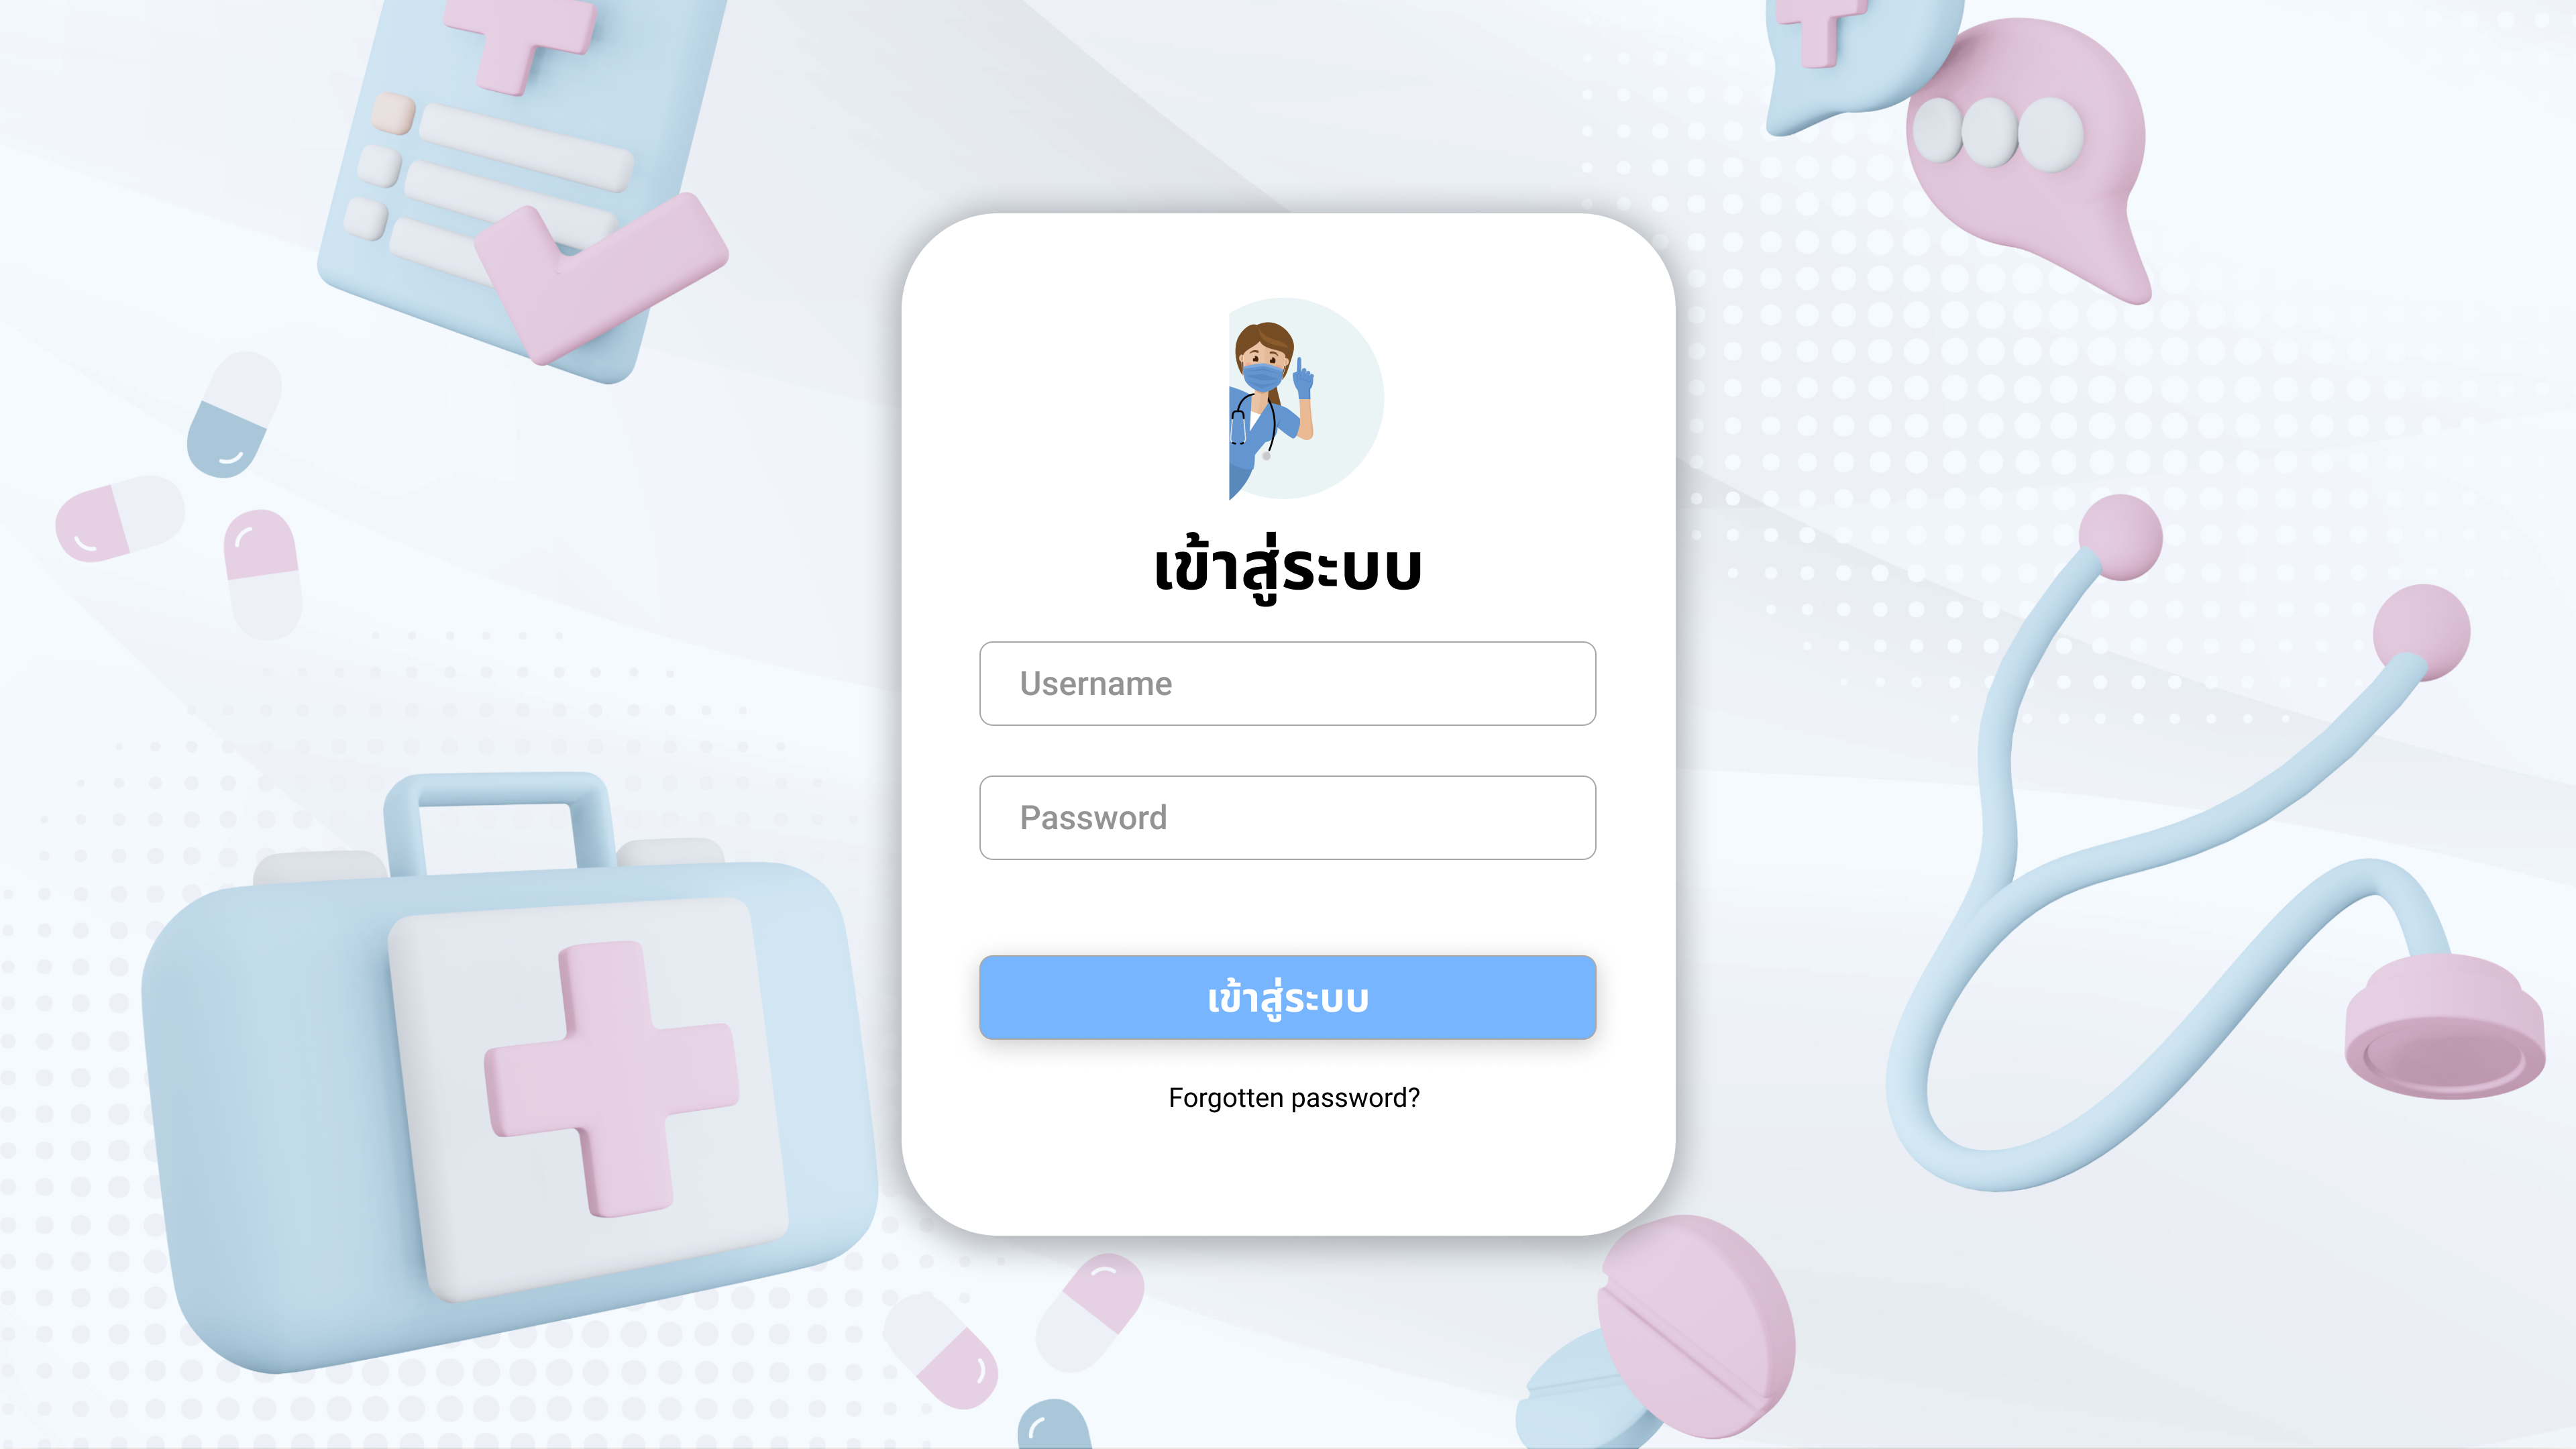
\includegraphics[width=0.6\textwidth]{Login ui.png}
    \caption{หน้าต่างการเข้าสู่ระบบของหัวหน้าพยาบาล}
    \end{figure}

\subsection{Nurse}

\begin{figure}[h]
    \centering
    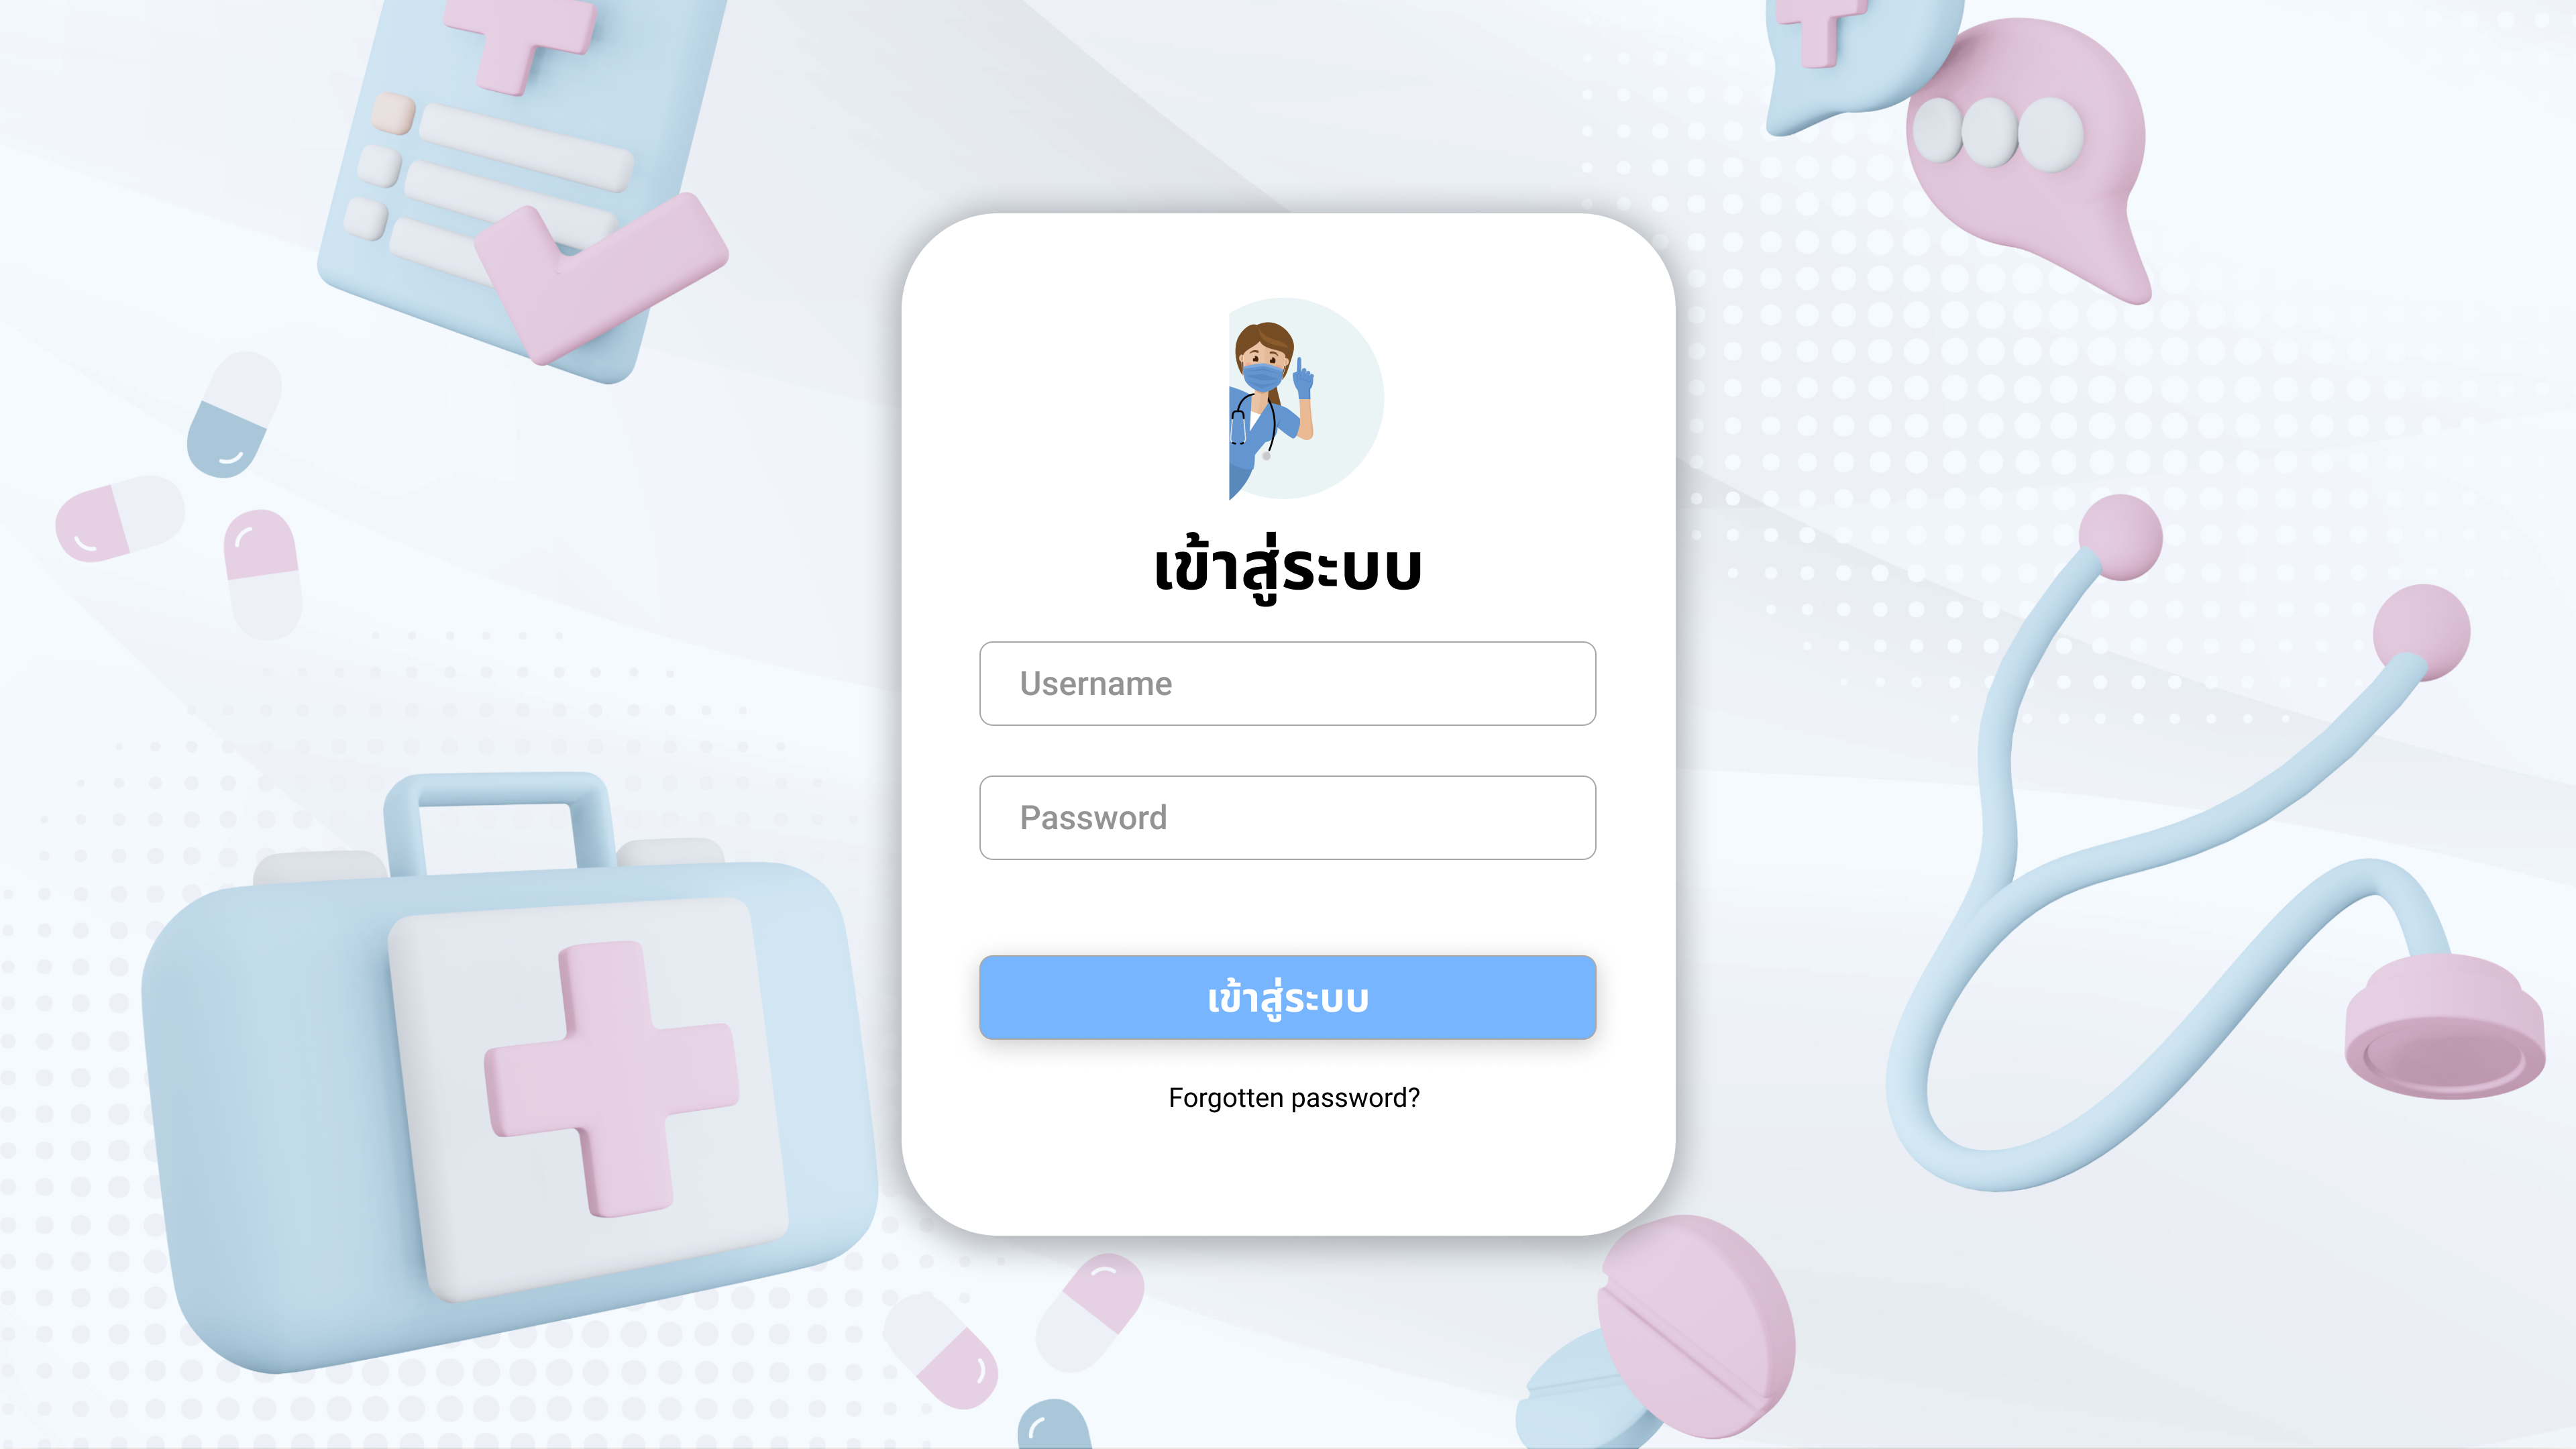
\includegraphics[width=0.6\textwidth]{Login ui.png}
    \caption{หน้าต่างการเข้าสู่ระบบของพยาบาล}
    \end{figure}

\begin{figure}
    \centering
    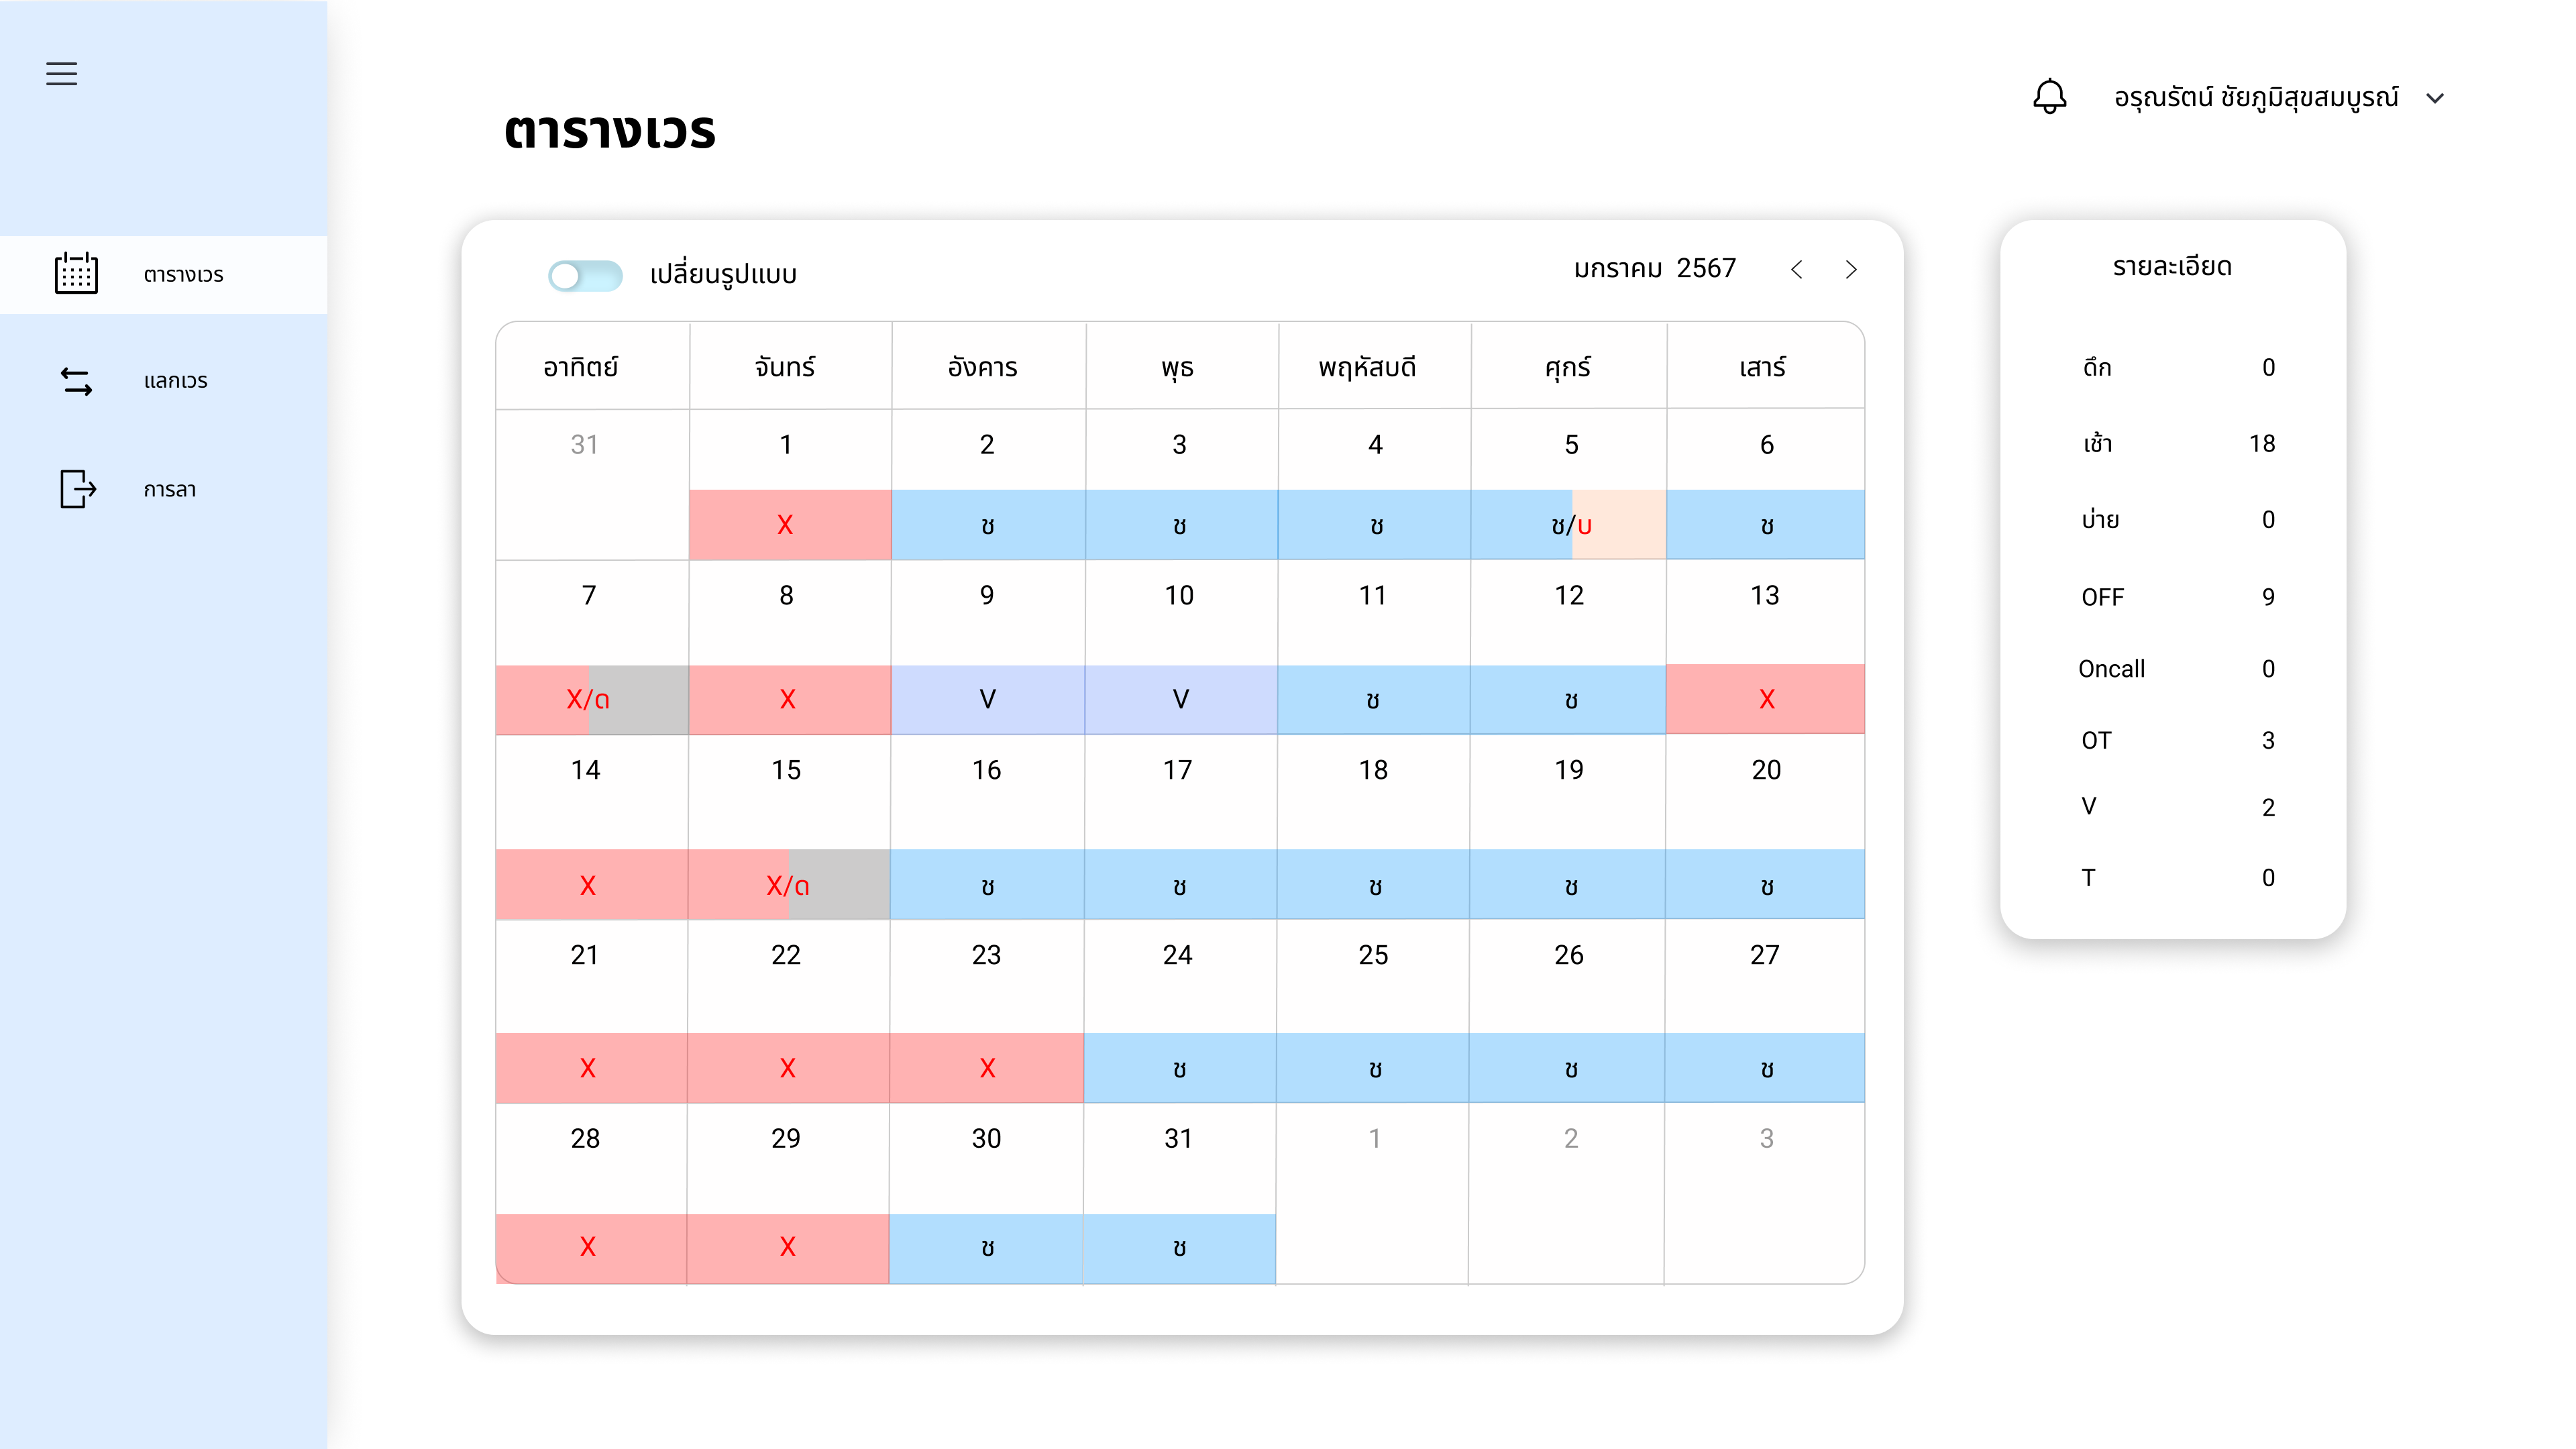
\includegraphics[width=0.6\textwidth]{Home ui.png}
    \caption{หน้าต่างหลักของพยาบาล}
\end{figure}
